\documentclass{beamer}

\usepackage{amsmath}
\usepackage{graphics}
\usepackage{framed}
\usepackage{amssymb}

\begin{document}
\begin{frame}
\textbf{\texttt{R} for Economic and Social Research}
\begin{enumerate}
\item \texttt{R} Packages and Taskviews, 10 packages
\item Official Statistics and Survey 
\item Regular Expressions with \texttt{R}
\item Econometric Tools: AER and Forecase
\item The HadleyVerse : ggplot and dplyr
\item Other Matters:  Julia and GitHub
\item Instructional Design : DataCamp
\end{enumerate}

\end{frame}
%=================================================================== %
MS4024 Numerical Computing Introduction to R Spring 2014
Contents
1 Introduction to R 3
1.1 Installing R . . . . . . . . . . . . . . . . . . . . . . . . . . . . . . . . . . . . . . 3
1.2 Command Line Interface . . . . . . . . . . . . . . . . . . . . . . . . . . . . . . . 3
1.3 The Assignment operator . . . . . . . . . . . . . . . . . . . . . . . . . . . . . . . 4
1.3.1 Reserved Words . . . . . . . . . . . . . . . . . . . . . . . . . . . . . . . . 4
1.4 Commenting . . . . . . . . . . . . . . . . . . . . . . . . . . . . . . . . . . . . . . 4
1.5 Defining Variables . . . . . . . . . . . . . . . . . . . . . . . . . . . . . . . . . . . 5
1.6 Help Functions . . . . . . . . . . . . . . . . . . . . . . . . . . . . . . . . . . . . 5
1.7 The help.start() command . . . . . . . . . . . . . . . . . . . . . . . . . . . . 5
1.8 Basic Maths Operations . . . . . . . . . . . . . . . . . . . . . . . . . . . . . . . 5
1.9 Basic R Editor . . . . . . . . . . . . . . . . . . . . . . . . . . . . . . . . . . . . 6
1.10 Built-In Data Sets . . . . . . . . . . . . . . . . . . . . . . . . . . . . . . . . . . 6
1.11 The summary() command . . . . . . . . . . . . . . . . . . . . . . . . . . . . . . 7
1.12 Working directories . . . . . . . . . . . . . . . . . . . . . . . . . . . . . . . . . . 7
1.13 Coming Unstuck . . . . . . . . . . . . . . . . . . . . . . . . . . . . . . . . . . . 7
1.14 Quitting the R environment . . . . . . . . . . . . . . . . . . . . . . . . . . . . . 8
1.15 Data Objects . . . . . . . . . . . . . . . . . . . . . . . . . . . . . . . . . . . . . 8
1.16 Listing all items in a workspace . . . . . . . . . . . . . . . . . . . . . . . . . . . 8
1.17 Removing items . . . . . . . . . . . . . . . . . . . . . . . . . . . . . . . . . . . . 8
1.18 Saving and Loading R Data Objects . . . . . . . . . . . . . . . . . . . . . . . . 8
2 Introduction to R (Continued) 9
2.1 Three particularly useful commands . . . . . . . . . . . . . . . . . . . . . . . . . 9
2.2 Changing GUI options . . . . . . . . . . . . . . . . . . . . . . . . . . . . . . . . 9
2.3 Colours . . . . . . . . . . . . . . . . . . . . . . . . . . . . . . . . . . . . . . . . 9
2.4 Use of the Semi-Colon Operator . . . . . . . . . . . . . . . . . . . . . . . . . . . 9
2.5 The apropos() Function . . . . . . . . . . . . . . . . . . . . . . . . . . . . . . . 9
2.6 History . . . . . . . . . . . . . . . . . . . . . . . . . . . . . . . . . . . . . . . . . 9
2.7 The sessionInfo() Function . . . . . . . . . . . . . . . . . . . . . . . . . . . . 10
2.8 Time and date functions . . . . . . . . . . . . . . . . . . . . . . . . . . . . . . . 10
2.9 Logical States . . . . . . . . . . . . . . . . . . . . . . . . . . . . . . . . . . . . . 10
2.10 Missing Data . . . . . . . . . . . . . . . . . . . . . . . . . . . . . . . . . . . . . 10
2.11 Files in the Working Directory . . . . . . . . . . . . . . . . . . . . . . . . . . . . 10
3 Inspecting a Data Set 11
3.1 Dimensions of a data set . . . . . . . . . . . . . . . . . . . . . . . . . . . . . . . 11
3.2 The summary() command . . . . . . . . . . . . . . . . . . . . . . . . . . . . . . 12
3.3 Structure of a Data Object . . . . . . . . . . . . . . . . . . . . . . . . . . . . . . 12
4 Packages 13
4.1 Packages . . . . . . . . . . . . . . . . . . . . . . . . . . . . . . . . . . . . . . . . 13
4.2 Using and Installing packages . . . . . . . . . . . . . . . . . . . . . . . . . . . . 13
4.2.1 Version of R . . . . . . . . . . . . . . . . . . . . . . . . . . . . . . . . . . 13
1MS4024 Numerical Computing Introduction to R Spring 2014
5 Data Creation, Data Entry, Data Import and Export 14
5.1 The c() command . . . . . . . . . . . . . . . . . . . . . . . . . . . . . . . . . . 14
5.1.1 Vector of Numeric Values . . . . . . . . . . . . . . . . . . . . . . . . . . 14
5.1.2 Vector of Character Values . . . . . . . . . . . . . . . . . . . . . . . . . . 14
5.1.3 Vector of Logical Values . . . . . . . . . . . . . . . . . . . . . . . . . . . 14
5.2 The scan() command . . . . . . . . . . . . . . . . . . . . . . . . . . . . . . . . 14
5.2.1 Characters with the scan() command . . . . . . . . . . . . . . . . . . . 15
5.3 Using the data editor . . . . . . . . . . . . . . . . . . . . . . . . . . . . . . . . . 15
5.4 Spreadsheet Interface . . . . . . . . . . . . . . . . . . . . . . . . . . . . . . . . . 15
2MS4024 Numerical Computing Introduction to R Spring 2014
\end{frame}
%==============================================================================================%
\begin{frame}

1 Introduction to R
Source: R project website (http://www.r-project.org)
R is a language and environment for statistical computing and graphics. It is a GNU project
which is similar to the S language and environment which was developed at Bell Laboratories
(formerly AT&T, now Lucent Technologies) by John Chambers and colleagues. R can be considered
as a different implementation of S. There are some important differences, but much
code written for S runs unaltered under R.
\end{frame}
%==============================================================================================%
\begin{frame}

R provides a wide variety of statistical (linear and nonlinear modelling, classical statistical tests,
time-series analysis, classification, clustering, ...) and graphical techniques, and is highly extensible.
The S language is often the vehicle of choice for research in statistical methodology,
and R provides an Open Source route to participation in that activity.
One of R’s strengths is the ease with which well-designed publication-quality plots can be
produced, including mathematical symbols and formulae where needed. Great care has been
taken over the defaults for the minor design choices in graphics, but the user retains full control.
R is available as Free Software under the terms of the Free Software Foundation’s GNU General
Public License in source code form. It compiles and runs on a wide variety of UNIX platforms
and similar systems (including FreeBSD and Linux), Windows and MacOS.
\end{frame}
%==============================================================================================%
\begin{frame}

R is a programming environment
• uses a well-developed but simple programming language
• allows for rapid development of new tools according to user demand
• these tools are distributed as packages, which any user can download to customize the R
environment.
\end{frame}
%==============================================================================================%
\begin{frame}

Base R and most R packages are available for download from the Comprehensive R Archive Network
(CRAN) cran.r-project.org. Base R comes with a number of basic data management,
analysis, and graphical tools R’s power and flexibility, however, lie in its array of packages
(currently more than 4,000!)
\end{frame}
%==============================================================================================%
\begin{frame}

1.1 Installing R
R is very easily installed by downloading it from the CRAN website. Installation usually takes
about 2 minutes. When Installation of R is complete, the distinctive R Icon will appear on your
desktop. To start R, simply click this Icon. It is common to re-install R once a year or so. The
current version of R, version 3.0.0. was released quite recently.
\end{frame}
%==============================================================================================%
\begin{frame}

1.2 Command Line Interface
When you start R, the command line interface window will appear on screen. This is one
of many windows in the R environment, others including graphical output windows, or script
3MS4024 Numerical Computing Introduction to R Spring 2014
editors. R code can be entered into the command line directly. Alternatively code can be saved
to a script, which can be run inside a session using the source() function.
\end{frame}
%==============================================================================================%
\begin{frame}

1.3 The Assignment operator
The assignment operator is used to assign names to particular values. Historically the assignment
operator was ) a ”<-”. The assignment operator can also be =. This is valid as of R
version 1.4.0.
Both will be used, although, you should learn one and stick with it. Many long term R
users prefer the arrow approach. You can also use -> as an assignment operator, reversing the
usual assignment positions. (This is actually really useful). Commands are separated either by
a semi colon or by a newline.
> a <- 6
> b = 5
> a + b ->c
> c
[1] 11
>e=7;f<-4
Before we continue, try using the up and down keys, and see what happens. Previously
typed commands are re-presented, and can be re-executed.
R stores both data and output from data analysis (as well as everything else) in objects.
The variables we have created so far are objects. A list of all objects in the current session can
be obtained with ls().
\end{frame}
%==============================================================================================%
\begin{frame}

1.3.1 Reserved Words
Some names are used by the system, e.g.T, F,q,c etc . Avoid using these.
\end{frame}
%==============================================================================================%
\begin{frame}
1.4 Commenting
For the sake of readability, it is good practice to comment code. The # character at the
beginning of a line signifies a comment, which is not executed. Lines of hashtags can be used
to identify the beginning and end of code segments
# This is a comment
#####################
# Start of Segment 1
#####################
4MS4024 Numerical Computing Introduction to R Spring 2014
\end{frame}
%==============================================================================================%
\begin{frame}
1.5 Defining Variables
A convention is to use define a variable name with a capital letter (R is case sensitive). This
reduces the chance of overwriting in-build R functions, which are usually written in lowercase
letters. Commonly used variable names such as x,y and z (in lower case letters) are not “reserved”.
\end{frame}
%==============================================================================================%
\begin{frame}

1.6 Help Functions
Help files for R functions are accessed by preceding the name of the function with ? (e.g. ?sort
). Alternatively you can use the command help() (e.g. help(sqrt) )
A HTML document appears on screen with information on the function typed in. As well
as the list of arguments that the particular function accepts, and how to specify them, there is
example code at the bottom of the file. These code segments are often invaluable in learning
how to master the function.

\end{frame}
%==============================================================================================%
\begin{frame}


1.7 The help.start() command
As mentioned by the text on the main console, the help.start() command can be usd to
access detailed help documentation that comes as part of the installation.
\end{frame}
%==============================================================================================%
\begin{frame}

1.8 Basic Maths Operations
The most commonly used mathematical operators are all supported by R. Here are a few
examples:
5 + 3 * 5 # Note the order of operations.
log (10) # Natural logarithm with base e=2.718282
log(8,2) # Log to the base 2
4^2 # 4 raised to the second power
7/2 # Division
factorial(4) #Factorial of Four
sqrt (25) # Square root
abs (3-7) # Absolute value of 3-7
pi # The mysterious number \\\
exp(2) # exponential function
\end{frame}
%==============================================================================================%
\begin{frame}

R can be used for many mathematical operations, including
• Set Theory
• Trigonometry
• Complex Numbers
• Binomial Coefficients
We will not go into any of these in great detail today.
5MS4024 Numerical Computing Introduction to R Spring 2014
\end{frame}
%==============================================================================================%
\begin{frame}

1.9 Basic R Editor
R has an inbuilt script editor. We will use it for this class, but there are plenty of top quality
Integrated Development Environments out there. (Read up about RStudio for example).
For these workshops, we will use the in-built script editor.
To start a new script, or open an existing script simply go to File and click the appropriate
options. A new dialogue box will appear. You can write and edit code using this editor.
To pass the code for compiling , press the run line or selection option (The third icon
on the menu).

\end{frame}
%==============================================================================================%
\begin{frame}

Another way to read code is to use the edit() function , which operates directly from the
command line. To see how the code defining an object X was written (or more importantly,
could have been written) simply type edit(X). This command has some useful applications
that we will see later on.
Scripts are saved as .R files. These scripts can be called directly using the source() command.

\end{frame}
%==============================================================================================%
\begin{frame}


1.10 Built-In Data Sets
Several data sets , intended as learning tools, are automatically installed when R is installed.
Many more are installed within packages to complement learning to use those packages. One
of these is the famous Iris data set, which is used in many data mining exercises.
• iris
• mtcars
• Nile

\end{frame}
%==============================================================================================%
\begin{frame}


To see what data sets are available, simply type data(). To load a data set, simply type in the
name of the data set. Some data sets are very large. To just see the first few (or last) rows, we
use the head() function or alternatively the tail() function. The default number of rows of
these commands is 6. Other numbers can be specified.
> head(iris)
Sepal.Length Sepal.Width Petal.Length Petal.Width Species
1 5.1 3.5 1.4 0.2 setosa
2 4.9 3.0 1.4 0.2 setosa
3 4.7 3.2 1.3 0.2 setosa
4 4.6 3.1 1.5 0.2 setosa
5 5.0 3.6 1.4 0.2 setosa
6 5.4 3.9 1.7 0.4 setosa
>
> tail(iris,4)
Sepal.Length Sepal.Width Petal.Length Petal.Width Species
147 6.3 2.5 5.0 1.9 virginica
148 6.5 3.0 5.2 2.0 virginica
149 6.2 3.4 5.4 2.3 virginica
150 5.9 3.0 5.1 1.8 virginic
\end{frame}
%==============================================================================================%
\begin{frame}
In many situations, it is useful to call a particular data set using the attach() command. This
will save having to specify the data sets over repeated operations. The file can then be detached
using the detach() command.
1.11 The summary() command

\end{frame}
%==============================================================================================%
\begin{frame}

The R command summary() is a generic function used to produce result “summaries” of the
results of various objects, from simple vectors to the output of complex model fitting functions.
The function invokes particular methods which depend on the class of the first argument.
> summary(Nile)
Min. 1st Qu. Median Mean 3rd Qu. Max.
456.0 798.5 893.5 919.4 1032.0 1370.0
>
> summary(Indometh)
Subject time conc
1:11 Min. :0.250 Min. :0.0500
4:11 1st Qu.:0.750 1st Qu.:0.1100
2:11 Median :2.000 Median :0.3400
5:11 Mean :2.886 Mean :0.5918
6:11 3rd Qu.:5.000 3rd Qu.:0.8325
3:11 Max. :8.000 Max. :2.7200
1.12 Working directories
You can change your working directly by using the appropriate options on the File menu. To
determine the current working directory, you can use the getwd() command. To change the
working directory , we would use the setwd() command. This is quite important as objects
will be imported and exported to and from the specified directory.
> getwd()
[1] "C:/Users/Kevin"
>
> setwd("C:/Users/Kevin/Documents")
>
> getwd()
[1] "C:/Users/Kevin/Documents"
1.13 Coming Unstuck
If you are having trouble with a piece of code that is currently compiling , all you have to do
is press ESC, just like many other computing environments.
7MS4024 Numerical Computing Introduction to R Spring 2014
1.14 Quitting the R environment
As the front page text indicates, all you have to do to quite the workspace is to type in q().
You will then be prompted to save your work.
\end{frame}
%==============================================================================================%
\begin{frame}

1.15 Data Objects
As mentioned previously, R saves data as objects. Examples of data objects are
• Vectors
• Lists
• Dataframes
• Matrices
The simple objects we have created previously are simply single element vectors.
\end{frame}
%==============================================================================================%
\begin{frame}

1.16 Listing all items in a workspace
To list all items in an R environment, we use the ls() function. This provides a list of all data
objects accessible. Another useful command is objects().
> ls()
[1] "a" "A" "authors" "b" "books"
[6] "C" "D" "ex1" "Gerb" "Lst"
[11] "m" "m1" "op" "presidents" "r"
[16] "showSmooth" "sm" "sm.3RS" "sm2" "sm3"
[21] "Trig" "Vec1" "x" "X" "x.at"
[26] "x1" "x2" "x3R" "y" "Y"
[31] "y.at"
\end{frame}
%==============================================================================================%
\begin{frame}

1.17 Removing items
Sometimes it is desirable to save a subset of your workspace instead of the entire workspace.
One option is to use the rm() function to remove unwanted objects right before exiting your R
session; another possibility is to use the save() function.

\end{frame}
%==============================================================================================%
\begin{frame}
1.18 Saving and Loading R Data Objects
In situations where a good deal of processing must be used on a raw dataset in order to prepare
it for analysis, it may be prudent to save the R objects you create in their internal binary form.
One attractive feature of this scheme is that the objects created can be read by R programs
running on different computer architectures than the one on which they were created, making it
very easy to move your data between different computers. Each time an R session is completed,
you are prompted to save the workspace image, which is a binary file called .RData in the
working directory.
\end{frame}
%==============================================================================================%
\begin{frame}
Whenever R encounters such a file in the working directory at the beginning of a session,
it automatically loads it making all your saved objects available again. So one method for
8MS4024 Numerical Computing Introduction to R Spring 2014
saving your work is to always save your workspace image at the end of an R session. If you
would like to save your workspace image at some other time during your R session, you can use
the save.image() function, which, when called with no arguments, will also save the current
workspace to a file called .RData in the working directory.
2 Introduction to R (Continued)
\end{frame}
%==============================================================================================%
\begin{frame}
2.1 Three particularly useful commands
1. help()
2. summary()
3. help.start()
2.2 Changing GUI options
We can change the GUI options using the GUI preferences option on the Edit menu. (Important
when teaching R) A demonstration will be done in class.
\end{frame}
%==============================================================================================%
\begin{frame}

2.3 Colours
R supported a massive number of colours. Type in colours() (or colors()) to see what colours
are supported.
2.4 Use of the Semi-Colon Operator
The semi-colon operator at the end of each line of code is not necessary in general, but using it
overcomes errors due to copying and pasting from document soft copies. In other programming
languages, such as Octave, using the semicolon in this way has a distinct purpose.
\end{frame}
%==============================================================================================%
\begin{frame}
2.5 The apropos() Function
This function is very useful for determining what functions are available for a particular topic,
although the process requires a great deal of trial and error. Suppose we are looking for a
command to compute the correlation coefficient. We would use a very short string (e.g. cor)
that would plausibly be part of useful function names.
apropos("cor")
\end{frame}
%==============================================================================================%
\begin{frame}

2.6 History
The command history() is used to obtain the last 25 commands used by R
history()
9MS4024 Numerical Computing Introduction to R Spring 2014
2.7 The sessionInfo() Function
To get a description of the version of R and its attached packages used in the current session,
we can use the sessionInfo() function
sessionInfo()
\end{frame}
%==============================================================================================%
\begin{frame}

2.8 Time and date functions
The commands Sys.time() and Sys.Date() returns the system’s idea of the current date
with and without time. We can perform some simple algebraic calculations to compute time
differences (i.e. to find out how long some code took to compile.
> X1=Sys.time()
> #Wait a few seconds
>
> X2=Sys.time()
> X2-X1 Time difference of 8.439614 secs
>
> Sys.Date() [1] "2012-09-01"
2.9 Logical States
Logical states TRUE and FALSE are simply specified as such, all in capital letters. The
shortcuts T and F are also recognized

\end{frame}
%==============================================================================================%
\begin{frame}


2.10 Missing Data
In some cases the entire contents of a vector may not be known. For example, missing data
from a particular data set. A place can be reserved for this by assigning it the special value
NA.
NA is a logical constant of length 1 which contains a missing value indicator. NA stands
for Not Available.

\end{frame}
%==============================================================================================%
\begin{frame}

2.11 Files in the Working Directory
It is possibel to call an R script from the working directory, using the source() function.
source("myfunctions.r")
source("mydata.r")
We can also send code put directly to a file in the working directory, using the sink()
command. The first time the command is used, the name of the created file is specified.
Subsequent commands print output directly to this file, until the command is used again to
cease the operation.
10MS4024 Numerical Computing Introduction to R Spring 2014
> sink("IrisSum.txt")
> summary(iris)
> sink()
>

\end{frame}
%==============================================================================================%
\begin{frame}

3 Inspecting a Data Set
• dim()
• nrow() and ncol()
• names()
• summary()
• tail()
• head()
• describe() (from the psych package)
\end{frame}
%==============================================================================================%
\begin{frame}

3.1 Dimensions of a data set
We have remarked that some data sets are very large. This is perhaps a good place to consider
summary information about data objects. For a simple vector, a useful command to determine
the length (remark: sample size) is the function length().
> Y=4:18
> length(Y)
[1] 15
For more complex data sets ( and data frames which we will see later) , we have several
tools for assessing the size of data.
> dim(iris) # dimensions of data set
[1] 150 5
> nrow(iris) # number of rows
[1] 150
> ncol(iris) # number of columns
[1] 5
11MS4024 Numerical Computing Introduction to R Spring 2014
We can also determine the row names and column names using the functions rownames()
and colnames(). If there are no specific row or column names, the command will just return
the indices.
> colnames(iris)
[1] "Sepal.Length" "Sepal.Width" "Petal.Length" "Petal.Width" "Species"

\end{frame}
%==============================================================================================%
\begin{frame}
3.2 The summary() command
The command summary() is one of the most useful commands in R. It is a generic function used
to produce result summaries of the results of various functions. The function invokes particular
methods which depend on the class of the first argument. In other words, R picks out the most
suitable type of summary for that data.
> summary(iris)
Sepal.Length Sepal.Width Petal.Length Petal.Width Species
Min. :4.300 Min. :2.000 Min. :1.000 Min. :0.100 setosa :50
1st Qu.:5.100 1st Qu.:2.800 1st Qu.:1.600 1st Qu.:0.300 versicolor:50
Median :5.800 Median :3.000 Median :4.350 Median :1.300 virginica :50
Mean :5.843 Mean :3.057 Mean :3.758 Mean :1.199
3rd Qu.:6.400 3rd Qu.:3.300 3rd Qu.:5.100 3rd Qu.:1.800
Max. :7.900 Max. :4.400 Max. :6.900 Max. :2.500
>
Summary is particularly useful for manipulating data from more complex data objects.
\end{frame}
%==============================================================================================%
\begin{frame}

3.3 Structure of a Data Object
The structure, class and storage mode of an object can be determined using the following
commands. Try out a few.
• str()
• class()
• mode()
> class(Nile)
[1] "ts"
> mode(Nile)
[1] "numeric"
>
> a
\end{frame}
%==============================================================================================%
\begin{frame}[1] 6
> mode(a)
[1] "numeric"
> class(a)
[1] "numeric"
> str(a)
num 6
>
> class(iris)
[1] "data.frame"
> mode(iris)
[1] "list"
\end{frame}
%==============================================================================================%
\begin{frame}
4 Packages
4.1 Packages
A Package in R is a file containing a collection of objects which have some common purpose.
Packages enhance the capabilties and scope for research in a certain field. For example the
package MASS contains objects associated with the Venables and Ripleys ”Modern Applied
Statistics with S”. Some examples of packages are Actuar, written for actuarial science, and
QRMlib, which complements the Quantitative Risk Management The command library()
lists all the available packages. To load a particular package, for example MASS, we would
write
library(MASS)

\end{frame}
%==============================================================================================%
\begin{frame}
4.2 Using and Installing packages
Many packages come with R. To use them in an R session, you need to load the package, as
previously demonstrated.
Some packages are not automatically installed when you install R but they need to be downloaded
and installed individually. We must first install them using the install.packages()
function, which typically downloads the package from CRAN and installs it for use. (follow the
instructions as indicated).
install.packages("ggplot2")
install.packages("qcc")
install.packages("sqldf")
install.packages("RMongo")
install.packages("randomforest")
\end{frame}
%==============================================================================================%
\begin{frame}
4.2.1 Version of R
Many packages will require you to have the most recent version of R and also other packages.
It is a good idea to update regularly.
13MS4024 Numerical Computing Introduction to R Spring 2014
5 Data Creation, Data Entry, Data Import and Export
\end{frame}
%==============================================================================================%
\begin{frame}
5.1 The c() command
To create a simple data set, known as a vector, we use the c() command to create the vector.
> Y=c(1,2,4,8,16 ) #create a data vector with specified elements
> Y
[1] 1 2 4 8 16
5.1.1 Vector of Numeric Values
Numvec = c(10,13,15,19,25);
5.1.2 Vector of Character Values
Charvec = c("LouLou","Oscar","Rasher");

\end{frame}
%==============================================================================================%
\begin{frame}
5.1.3 Vector of Logical Values
Charvec = c(TRUE,TRUE,FALSE,TRUE);

Vectors can be bound together either by row or by column.
> X=1:3; Y=4:6
> cbind(X,Y)
X Y
[1,] 1 4
[2,] 2 5
[3,] 3 6
>
> rbind(X,Y)
[,1] [,2] [,3]
X 1 2 3
Y 4 5 6
\end{frame}
%==============================================================================================%
\begin{frame}
5.2 The scan() command
The scan() function is a useful method of inputting data quickly. You can use to quickly copy
and paste values into the R environment. It is best used in the manner as described in the
following example. Create a variable ”X” and use the scan() function to populate it with
values. Type in a value, and then press return. Once you have entered all the values, press
return again to return to normal operation.
> X=scan()
1: 4
2: 5
14MS4024 Numerical Computing Introduction to R Spring 2014
3: 5
4: 6
5:
Read 4 items
Remark: Try the edit() command on object X.
5.2.1 Characters with the scan() command
The scan() command can also be used forinputting character data.
> Y=scan(what=" ")
1: LouLou
2: Oscar
3: Rasher
4:
Read 3 items
> Y
[1] "LouLou" "Oscar" "Rasher"
\end{frame}
%==============================================================================================%
\begin{frame}
5.3 Using the data editor
5.4 Spreadsheet Interface
R provides a spreadsheet interface for editing the values of existing data sets. We use the
command data.entry(), and name of the data object as the argument. (Also try out the
fix() command)
> data.entry(X) # Edit the data set and exit interface
> X
\end{frame}
%==============================================================================================%
\begin{frame}
% % SLIDE 1 - COVER SLIDE
\begin{figure}
\centering

\includegraphics[width=0.7\linewidth]{Rlogo}
\end{figure}
\LARGE
\[ \mbox{Using R for Economic and Social Research} \]	



\end{frame}



%=================================================================== %
\begin{frame}[fragile]
	
	
	\begin{figure}
\centering
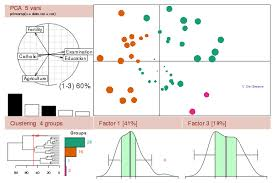
\includegraphics[width=0.7\linewidth]{CRAN}
\caption{Comprehensive R Archive Network}

\end{figure}
	
	
\end{frame}



%=================================================================== %
\begin{frame}[fragile]
	
\frametitle{Packages}
\begin{itemize}
\item The CRAN package repository features 6107 available packages. 
\item Packages contain
various functions and data sets for numerous purposes, e.g.
\textbf{\textit{ggplot2}} package, \textbf{\textit{AER}} package, \textbf{\textit{survival}} package, etc.
\item Some packages are part of the basic installation. Others can be
downloaded from CRAN.
\item To access all of the functions and data sets in a particular package,
it must be loaded into the workspace. 
\item For example, to load the
\textbf{\textit{ggplot2}} package:
\end{itemize}
\begin{framed}
\begin{verbatim}
install.packages(ggplot2)
library(ggplot2)
\end{verbatim}
\end{framed}
\end{frame}
%=================================================================== %
\begin{frame}	
\frametitle{R Packages}

\begin{itemize}
\item ``10 R packages I wish I knew about earlier" - Drew Conway (Yhat.com, February 2013)
\bigskip \item ``The HadleyVerse" - Hadley Wickham
\begin{itemize}
	
	\item  ggplot2, dplyr, reshape, lubridate, stringr
	
	\item  With Romain Francois, Dianne Cook and Garret Grolemund.
\end{itemize}
\bigskip
\item Dr Brendan Haplin (UL): lme4 ,TraMineR, Gelman's arm, MASS, foreign. 
\bigskip
\item Shiny - Web Applications with \texttt{R}
\end{itemize}
\end{frame}



%=================================================================== %
\begin{frame}
\frametitle{The forecast Package}	
	
forecast makes it incredibly easy to fit time series models like ARIMA, ARMA, AR, Exponential Smoothing, etc.

	
	
\end{frame}


%=================================================================== %
\begin{frame}
	\frametitle{The forecast Package}	
	
	\begin{figure}
\centering
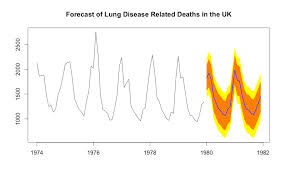
\includegraphics[width=0.7\linewidth]{forecast}

\end{figure}

	
	
\end{frame}
%=================================================================== %
\begin{frame}
	
	
	
	
	\begin{figure}
\centering
\includegraphics[width=0.9\linewidth]{ggplotdensity}
\caption{}
\label{fig:ggplotdensity}
\end{figure}

\end{frame}





%=================================================================== %
\begin{frame}
	
	
	
	
	\begin{figure}
\centering
\includegraphics[width=0.45\linewidth]{"ASDAbook cover"}
\caption{Springer's UseR! series}
\end{figure}

\end{frame}
%=================================================================== %
\begin{frame}[fragile]
\Large
\begin{framed}
\begin{verbatim}
"As usual, NZ is ahead of the pack and 
@statisticsnz is the first govt 
statistics agency to deploy 
rstudio server pro! #rstats"

                      Hadley Wickham, 
                      (11th December).
\end{verbatim}
\end{framed}

\end{frame}

	
%ESRItalk
\begin{frame}[fragile]
The American Community Survey distributes downloadable data about United States communities. 
Download the 2006 microdata survey about housing for the state of Idaho using \texttt{download.file()} from here: 

\begin{verbatim}
https://dl.dropbox.com/u/7710864/data/csv_hid/ss06hid.csv

or here:

https://spark-public.s3.amazonaws.com/dataanalysis/ss06hid.csv 
\end{verbatim}
and load the data into \texttt{R}. 
\end{frame}
%=========================================================================== %

% You will use this data for the next several questions. 
\begin{frame}[fragile]
\noindent \textbf{\textit{Code Book}}\\
The code book, describing the variable names is here: 

\begin{verbatim}
https://dl.dropbox.com/u/7710864/data/PUMSDataDict06.pdf

or here: 

https://spark-public.s3.amazonaws.com/dataanalysis/PUMSDataDict06.pdf
\end{verbatim}
\end{frame}
%=========================================================================== %
\begin{frame}[fragile]

How many housing units in this survey were worth more than \$1,000,000?
% **53**

%\begin{framed}
%	\begin{verbatim}
%	# Download 2006 microdata survey 
%	# re: housing for Idaho using download.file()
%	# setwd("~/DA")
%	download.file(
%	'https://spark-public.s3.amazonaws.com/dataanalysis/ss06hid.csv',
%	"ss06hid.csv", method="curl")
%	
%	# Download the code book:
%	# download.file(
%	'https://spark-public.s3.amazonaws.com/dataanalysis/PUMSDataDict06.pdf',
%	"PUMSDataDict06.pdf", method="curl")
%	\end{verbatim}
%\end{framed}

\end{frame}

%=========================================================================================== %

\begin{frame}[fragile]

\begin{framed}
	\begin{verbatim}	
	# load the data into R
	idahoData <- read.csv("ss06hid.csv", header=TRUE)
	
	# Is it just Idaho data?
	table(idahoData$ST)
	#Check the PDF - what does 16 mean?
	
	#any missing data?
	summary(idahoData$ST)
	
	# How many housing units are worth
	# more than $1,000,000?
	table(idahoData$TYPE,idahoData$VAL)
	\end{verbatim}
\end{framed}

\end{frame}

%=========================================================================================== %

\begin{frame}[fragile]

\begin{framed}
	\begin{verbatim}
	#from local files
	idahoData <- read.csv("daquiz2.csv", header=TRUE)
	
	\end{verbatim}
\end{framed}

\end{frame}

%=========================================================================================== %

\begin{frame}[fragile]
\frametitle{Question 4}

\begin{itemize}
	\item Use the data you loaded from Question 3. 
	\item Consider the variable FES. 
	\item Which of the "tidy data" principles does this variable violate?
\end{itemize}

%%READY
%\textbf{\textit{Revision}}\\
%What are the three characteristics of tidy data?
%
%\begin{itemize}
%	\item ``\textit{\textbf{Tidy data}}" by Hadley Wickham (RStudio)
%	\item Submission to Journal of Statistical Software
%	\item (http://vita.had.co.nz/papers/tidy-data.pdf)
%\end{itemize}
%Three Principles from Hadley Wickham's paper
%\begin{itemize}
%	\item[1.] Each variable forms a column, 
%	\item[2.] Each observation forms a row, 
%	\item[3.] Each table/file stores data about one kind of observation.
%\end{itemize}

\begin{framed} 
	\begin{verbatim}
	# let's look!
	unique(idahoData$FES)
	\end{verbatim}
\end{framed} 

\end{frame}
%-----------------------------------------------------------------%

%\subsection*{ Question 5 }
\begin{frame}


\textbf{Options}
\begin{itemize}
	\item[(i)]  Each tidy data table contains information about only one type of observation.\\
	(Not so)
	
	\item[(ii)]  Each variable in a tidy data set has been transformed to be interpretable.
	(No)
	
	\item[(iii)]  Tidy data has no missing values.
	
	\item[(iv)]  Tidy data has one variable per column.
\end{itemize}
\end{frame}
%-----------------------------------------------------------------%

%\subsection*{ Question 5 }
\begin{frame}[fragile]
Use the data you loaded from Question 3. 

\begin{itemize}
	\item How many households have 3 bedrooms and and 4 total rooms? 
	\item How many households have 2 bedrooms and 5 total rooms? 
	\item How many households have 2 bedrooms and 7 total rooms?
\end{itemize}
\begin{framed}
	\begin{verbatim}
	#USING TABLE
	#Rooms on Rows , Bedrooms on Columns
	#dnn adds dimension names
	
	table(idahoData$RMS,idahoData$BDS,dnn=list("RMS","BDS"))
	
	\end{verbatim}
\end{framed}

\end{frame}
%============================================================= %
\begin{frame}[fragile]
Another Way of Doing it
\begin{framed}
	\begin{verbatim}
	# How many households have 3 bedrooms and 4 total rooms?
	nrow(idahoData[!is.na(idahoData$BDS) & idahoData$BDS==3 &
	!is.na(idahoData$BDS) & idahoData$RMS==4,])
	# How many households have 2 bedrooms and 5 total rooms?
	nrow(idahoData[!is.na(idahoData$BDS) & idahoData$BDS==2 &
	!is.na(idahoData$BDS) & idahoData$RMS==5,])
	# How many households have 2 bedrooms and 7 total rooms?
	nrow(idahoData[!is.na(idahoData$BDS) & idahoData$BDS==2 &
	!is.na(idahoData$BDS) & idahoData$RMS==7,])
	
	\end{verbatim}
\end{framed}
% **148, 386, 49**
\end{frame}

%-----------------------------------------------------------------%

%\subsection*{Question 6}
\begin{frame}
\begin{itemize}
	\item Use the data from Question 3. 
	\item Create a logical vector that identifies the households on greater than 10 acres who sold more than \$10,000 worth of agriculture products. 
	\item Assign that logical vector to the variable `\texttt{agricultureLogical}`. 
	\item Apply the `\texttt{which()} function like this to identify the rows of the data frame where the logical vector is `TRUE`.
\end{itemize}

\end{frame}
%====================================================== %
\begin{frame}[fragile]
\begin{framed} 
	\begin{verbatim}
	# Like this (this wont run yet)
	which(agricultureLogical) 
	\end{verbatim}
\end{framed} 
\end{frame}
%====================================================== %
\begin{frame}[fragile]
What are the first 3 values that result?

\begin{framed} \begin{verbatim}
	# Showing off a bit
	q6cols <- c("ACR", "AGS")
	which(names(idahoData) %in% q6cols)  
	
	# logical vector
	agricultureLogical <- idahoData$ACR==3 & idahoData$AGS==6
	
	# and:
	which(agricultureLogical) 
	\end{verbatim}\end{framed} 

%**125, 238, 262**
\end{frame}
%====================================================== %
\begin{frame}
	
\frametitle{Question 7}

\begin{itemize}
	\item Use the data from Question 3. 
	\item Create a logical vector that identifies the households on greater than 10 acres who
	sold more than \$10,000 worth of agriculture products. 
	\item Assign that logical vector to the variable \texttt{agricultureLogical}. 
	\item Apply the \texttt{which()} function like this to identify the rows of the 
	data frame where the logical vector is TRUE and assign it to the variable indexes. 
\end{itemize}

\end{frame}
%====================================================== %
\begin{frame}[fragile]
	
\begin{framed} 
\begin{verbatim}
	indexes =  which(agricultureLogical) 
\end{verbatim}
\end{framed} 

If your data frame for the complete data is called \texttt{dataFrame} you can create a data frame 
with only the above subset with the command: 

\end{frame}
%====================================================== %
\begin{frame}[fragile]
	
\begin{framed} 
	\begin{verbatim}
	subsetDataFrame  = dataFrame[indexes,] 
	\end{verbatim}
\end{framed} 

\noindent Note that we are subsetting this way because the NA values in the variables 
will cause problems if you subset directly with the logical statement. 

\end{frame}
%====================================================== %
\begin{frame}[fragile]
	
\noindent How many households in the subsetDataFrame have a missing value for the mortgage status 
(MRGX) variable?

\begin{framed} 
	\begin{verbatim}
	indexes <- which(agricultureLogical)
	subsetIdahoData <- idahoData[indexes,]
	
	# And then:
	nrow(subsetIdahoData[is.na(subsetIdahoData$MRGX),])
	\end{verbatim}
\end{framed} 

\end{frame}
%====================================================== %
\begin{frame}[fragile]
	
\frametitle{Question 8}
\begin{itemize}
	\item Use the data from Question 3.
	\item Apply `\texttt{strsplit()}` to split all the names of the data frame on the characters "wgtp". 
	\item What is the value of the 123 element of the resulting list?
\end{itemize}

\begin{framed} \begin{verbatim}
	List <- strsplit(names(idahoData), "wgtp")
	List[123]
	\end{verbatim}\end{framed} 

%**"" "15"**
\end{frame}
%====================================================== %
\begin{frame}[fragile]
\frametitle{Question 9}

What are the 0\% and 100\% quantiles of the variable \texttt{YBL}? Is there anything wrong with these values?
\textit{ Hint: you may need to use the \texttt{na.rm} parameter.}

\begin{framed} 
	\begin{verbatim}
	quantile(idahoData$YBL, na.rm=TRUE)
	#  0%  25%  50%  75% 100% 
	#  -1    3    5    7   25 
	\end{verbatim}
\end{framed} 

\end{frame}
%====================================================== %
\begin{frame}[fragile]	
\frametitle{Question 10}

In addition to the data from Question 3, the American Community Survey also collects data about populations. 
Using `\texttt{download.file()}`, download the population record data from: 

\begin{verbatim}
https://dl.dropbox.com/u/7710864/data/csv_hid/ss06pid.csv 

or here:

https://spark-public.s3.amazonaws.com/dataanalysis/ss06pid.csv
\end{verbatim}

\end{frame}
%====================================================== %
\begin{frame}[fragile]
	
\begin{itemize}
	\item Load the data into \texttt{R}. Assign the housing data from Question 3 to a data frame `\texttt{housingData}` and the population data from above to a data frame `populationData`.
	
	\item Use the merge command to merge these data sets based only on the common identifier "SERIALNO". 
	
	\item What is the dimension of the resulting data set? 
\end{itemize}
%[OPTIONAL] For fun, you might look at the data and see what happened when they merged.

\end{frame}
%========================================================================================== %
\begin{frame}[fragile]
	
%	download.file(
%	'https://spark-public.s3.amazonaws.com/dataanalysis/ss06pid.csv',
%	'ss06pid.csv', method='curl')
%	
\textbf{Merging Data Sets}
\begin{framed} 
	\begin{verbatim}

	housingData <- read.csv("ss06hid.csv", header=TRUE)
	popuData <- read.csv("ss06pid.csv", header=TRUE)
	
	dim(merge(housingData, 
	popuData, by="SERIALNO", all=TRUE))
	\end{verbatim}
\end{framed} 

\end{frame}
% **number of rows = 15451, number of columns = 426**

\end{document}
